\documentclass[12pt]{report}
\usepackage{graphicx}
\usepackage{algorithm}
\usepackage{algorithmic}

\usepackage{pdfcomment}
\newcommand{\note}[1]{\raisebox{0pt}[0pt][0pt]{\pdfcomment[open=true]{#1}}}

% [dme] reordered these document definitions - title, author, date -
% if they sit here, they can potentially use the macros you include
% from packages
\title{Avoiding the Dark Side}
\author{
        Leslie Chisholm \\
                Department of Computer Science\\
}
\date{\today}

\begin{document}
\maketitle

\begin{abstract}
This is the paper's abstract \ldots
\end{abstract}

\tableofcontents
\listoffigures\
\listofalgorithms
\chapter{Introduction}
The city of Dunedin is well known for being a dark and cold city because of the hills surrounding the centre of the city that shade large areas in the winter months. This project set out to discover the amount of sunlight Dunedin receives over any given period of the year and present the data in a way that a user could use it to draw conclusions from.

\section{Goals}
The goals of this project were research and implement a sunlight projection model for the city of Dunedin. There are two parts; an interactive three-dimensional display to show point in time distribution of sunlight over Dunedin and a data aggregator to augment the display with computed measures of sunlight coverage over time ranges.

\section{Chapter outline}
The chapters in this report will be written in the order in which they were completed. Chapter two focuses on how physical data was gathered from the environment, the methods used to convert them into a representation usable for the project and the accuracy that was obtained in these measurements. Chapter three looks at the interactive three-dimensional viewer built to display the distribution of sunlight over Dunedin in real-time and it is implemented using OpenGL and JOGL. Chapter four is about the data aggregator, which accurately calculates the amount of sunlight an area receives, how its output can be viewed in the viewer or output to a Targa image or comma separated value file, and the results generated by it.
In chapter x y will be presented...

\section{Background Information}
\subsection{OpenGL and JOGL} 
To create the viewer and allow it to be used in an interactive method the Java OpenGL (JOGL)\cite{JOGL} libraries are used. JOGL is a wrapper library that exports the OpenGL application programming interface (API) to the Java programming language. OpenGL or Open Graphics Library is a cross platform API for writing applications that use two and three dimensional computer graphics. The project uses version 2.0 of the OpenGL libraries for access to programmable shaders and buffer objects and will be able to run on any graphics hardware that supports OpenGL 2.0.

\note{Does `Background' normally sit in the introduction chapter? In a PhD thesis it would usually be chapter two. The problem with having it here is that the chapter outline comes after it. In most theses I've seen (these are not 480 project reports though) only the introduction text would come before the chapter outline. Hmm ok I've moved it to be after the chapter outline. I don't think a whole chapter could be taken up with background information}


\chapter{Physical Data}

A digital elevation model of Dunedin and a mathematical model of the sun's position were gathered. The digital elevation model is used to generate the three-dimensional map of Dunedin 


\section{Elevation Data}
\begin{figure}
\caption{The Height Map generated from the Data and shown in 3D in the viewer}
\label{elevation}
\end{figure}

The height data for Dunedin was collected from the surveying department of the University of Otago. The data contains a map with a width of 1237 points and a height of 881 points and covers most of general Dunedin from South Taieri to the top of Pine Hill. The data is encoded as a 1237x881 text file of decimal pointed numbers that represent the height above sea level of that point. The resolution of the data is 20 metres between points. There are areas where the data is less accurate, such as the hills West of Leith Valley and around Cape Saunders, and the water.

\begin{figure}
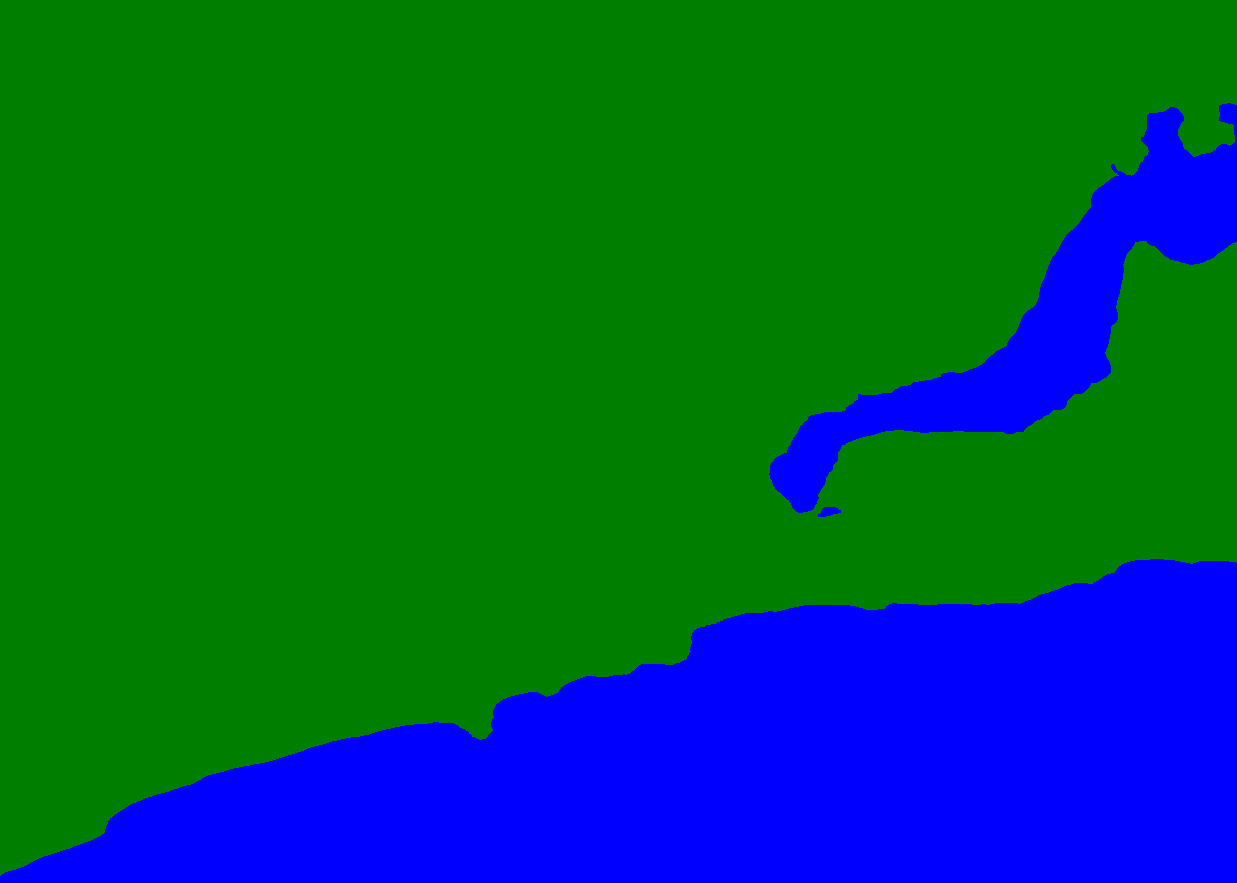
\includegraphics[scale=0.4]{terrain.png}
\caption{Water texture}
\label{overlaytexture}
\end{figure}
To work around the inaccuracies in the water level an image was generated \ref{overlaytexture} with the areas of water coloured blue and the areas of land that the aggregator is not looking at coloured black. The image is overlayed on the height data map with a 1:1 mapping to show what areas of land are in water. Areas of land are clamped to a height of 0.1 if they are within water. 

Before a water overlay texture was being used any land below zero metres was assumed to be below sea level. Doing this caused problems in areas of reclaimed land such as South Dunedin and the harbour area being thought of as below sea level. 

 Generating this image was also useful when running the aggregator because the water is already clearly marked on the map and thus areas in the water can be safely ignored to get a speed bonus. 

\subsection{Accuracy}
To test the accuracy of the height data a global positioning system (GPS) was to be used to check the accuracy of the height points however this turned out to be infeasible because the accuracy of the GPS's height data was far lower than expected and to inaccurate to be included in the project. A GPS is rated to be accurate to approximately +/- 15 metres 95\% of the time\cite{gpsaltitude}. The inaccuracies were observed when standing at sea level with a GPS and getting results approximately 10 metres higher than the current position.

The best way to confirm the accuracy of the height data would be to compare it to other geographical data sources. Before going to the surveying department for the height information other sources were tried. The Shuttle Radio Topography Mission (SRTM)\cite{srtm} was a near-global scale project by NASA to generate topographical maps and includes all of New Zealand at a resolution of 30 metres. A old version of ARC GIS was provided by Geoff Wyvill containing topographical information about New Zealand, unfortunately the software to read the topographical maps was quite old and could not be run on any of the operating systems there was access to in the department.

\subsection{Future Work}
Unfortunately time constraints meant that there was not enough time to explore these methods of collecting height data and compare them to the height data.
 Given more time these data sources could be thoroughly explored and a larger collection of geographical data collected and utilised within the project, allowing the user to examine more cities than Dunedin.

\section{Sun}
To generate shadows over the representation given of Dunedin the sun's position has to be calculated accurately using the current time and geographical position.


\subsection{Calculating the Position of the Sun}
To calculate the position of the sun code from the RedShift project\cite{redshift} was used to ensure that the code had been previously tested. Code from other projects were examined, such as the solar positioning libraries for Java\cite{javasunlib} however the algorithms used in this library, the PSA\cite{psa} and SPA\cite{spa} algorithms, have the unfortunate downside that they do not work for areas in the Southern Hemisphere and modifying the algorithms used in their papers are outside the scope of the project.

The code modified from the RedShift library are the solar.c and solar.h files, which are taken from javascript code by U.S. Department of Commerce, National Oceanic & Atmospheric Administration\cite{usnoaa} and is based on equations from Astronomical Algorithms\cite{astronomicalalgorithms}.

\subsection{Calculating the Sunrise and Sunset}
Calculations of the sunset and sunrise times taken from \cite{sunrise} 
\subsection{Sun Accuracy}
\begin{figure}
\caption{Device used to accurately calculate the position of the sun}
\label{sun-contraption}
\end{figure}
The accuracy of the sun was tested by comparing the results from the algorithms used in the project and by other sun position calculators and by creating a device to calculate the position of the sun at the current time.

\chapter{Viewer}
\begin{figure}[h]
\centering
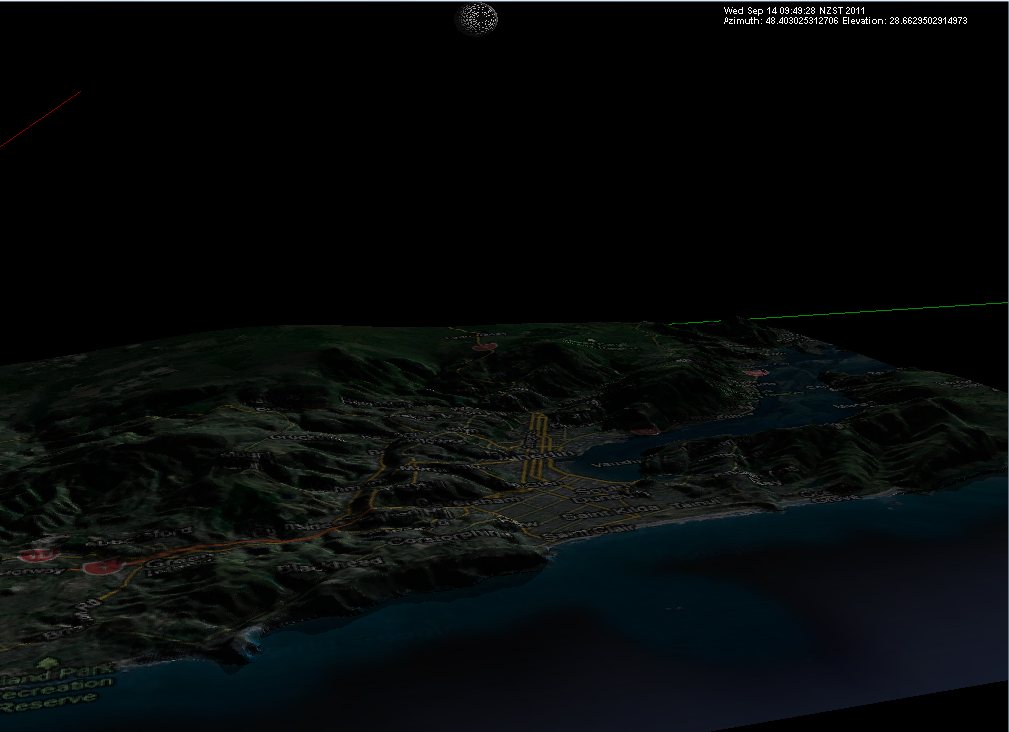
\includegraphics[scale=0.4]{viewer.png}
\caption{A screenshot of the viewer looking down at Dunedin}
\end{figure}\note{Good to see the screenshot! :-) Can the brightness/contrast be adjusted? It is very dark on my system.}
The viewer is an interactive three-dimensional simulator of the Sun moving over Dunedin. It allows the user to view shadows cast by the sun over the varying landscape. It exposes the ability to run in two different modes; shadow-mapping mode, where OpenGL shadow maps are used to generate shadows, and aggregator shadowing mode, where the shadow data from the aggregator is used to calculate shadows. This chapter will focus mostly on the OpenGL and shadow mapping side of the viewer.

\section{Drawing the elevation data}
Geographical height data is drawn by the viewer using OpenGL. After the height data has been gathered by the program OpenGL buffer objects are created to store the vertex position,colour, texture coordinates and vector normals. Buffer objects allow sending the data to be drawn directly to the graphics cards local memory where it can be redrawn and updated quickly without unnecessary resending. Due to the large number vertices present in the height data and the static nature of the data using buffers to store the data lowers the number of graphics hardware calls significantly in comparison to using the fixed function pipeline.

\section{Shadows}
Shadows are done on the graphics hardware using shadow maps...
\section{Usage}
The viewer can be run on any computer with a reasonably new graphics processor...
\subsection{Control}
The viewer can be controlled using the \texttt{w},\texttt{a},\texttt{s},and \texttt{d} keys to zoom in and out and mouse drags to rotate the screen...
\section{Future Work}
\chapter{Aggregator}
The aggregator is designed to calculate whether a portion of land is in shadow or not more accurately then using OpenGL methods such as shadow mapping...
\section{Algorithms Used}
A modified version of Cleary's algorithm was used to calculate whether a given block of land is in shadow or not... See algorithm~\ref{alg:shadow-calculation} for more information... \note{very nice! Always use named references though. I've fixed this instance.}

\begin{algorithm}[h]                      % enter the algorithm environment
\caption{Calculate whether a given point is in shadow or not}          % give the algorithm a caption
\label{alg:shadow-calculation}                           % and a label for \ref{} commands later in the document
\begin{algorithmic}                    % enter the algorithmic environment
\REQUIRE $n \geq 0 \vee x \neq 0$
\ENSURE $y = x^n$
\STATE $y \Leftarrow 1$
\IF{$n < 0$}
\STATE $X \Leftarrow 1 / x$
\STATE $N \Leftarrow -n$
\ELSE
\STATE $X \Leftarrow x$
\STATE $N \Leftarrow n$
\ENDIF
\WHILE{$N \neq 0$}
\IF{$N$ is even}
\STATE $X \Leftarrow X \times X$
\STATE $N \Leftarrow N / 2$
\ELSE[$N$ is odd]
\STATE $y \Leftarrow y \times X$
\STATE $N \Leftarrow N - 1$
\ENDIF
\ENDWHILE
\end{algorithmic}
\end{algorithm}

\section{Optimisations}
The aggregator can run faster by checking for shadows at the edges of an area of land. If there is no shadow present at any of the edges then it is safe to assume that none of the points within that region will be in shadow...\note{Good. Well expressed, too. Perhaps mention that there are more general forms of this optimisation strategy, but that there will be a cross-over point between the efficiency gained by not computing shadow rays against the extra effort in running the optimisation algorithm.}
\section{Data Gathered}
By running the aggregator for the whole year it was seen that suburb x managed to receive the highest amount of sun...
\section{Future work}
\chapter{Conclusion}
In the end the project was able to do x well and didn't do y as well as expected.
\bibliographystyle{abbrv}
\bibliography{480}

\end{document}
